\PassOptionsToPackage{quiet}{fontspec} % 抑制中文字体警告

\documentclass[12pt,AutoFakeSlant,AutoFakeBold]{article}
\usepackage{ctex}
\usepackage[a4paper,top=2.5cm,bottom=2.5cm,left=2.5cm,right=2.5cm]{geometry}

% Useful packages
\usepackage{amsmath}
\usepackage{amsfonts,amssymb}
\usepackage{graphicx}
\usepackage[colorlinks=true, allcolors=blue]{hyperref}
\usepackage{booktabs}
\usepackage{subfig}
\usepackage{enumitem}
\usepackage{minted}
\usepackage{titlesec}
\usepackage{amsfonts}
\usepackage{longtable}
\usepackage{gbt7714}
\usepackage{mdwlist}
\usepackage{listings}
\usepackage{float}
\usepackage{svg}
\svgsetup{inkscapelatex = false}
\titleformat*{\section}{\Large\itshape\centering}

\title{体内药物浓度随时间的变化规律}
\author{软件2204 徐翌森 2183214655}

\begin{document}

\maketitle

\centerline{\large\heiti\textbf{摘要}}

处方药的超剂量可能会对患者造成严重的负面影响,甚至导致死亡;而剂量不足则无法达到预期的治疗效果。本文针对药物浓度的衰减速度与正比与药物浓度的一类药物进行了分析。我们给出了在给定单次服药量$A$,服药间隔$T$与药物衰减系数$k$的情况下,病人体内药物浓度随时间变化的曲线。

然后,我们通过分析数列的极限,得到了在足够长时间后,药物在病人体内的浓度将会在$\frac{A\,\mathrm{e}^{-k\,T}}{1 - \mathrm{e}^{-k\,T}}$到$\frac{A}{1 - \mathrm{e}^{-k\,T}}$之间波动。

最后,我们假定,药物在体内的合理浓度为从$C_{min}$到$C_{max}$,那么我们可以解出,服药周期$T$需要满足的关系:
\begin{equation*}
    0 < T \leq -\frac{\ln\frac{C_{min}}{C_{max}}}{k}
\end{equation*}
对于任意一个给定的$T$,我们也可以得到单次服药量$A$需要满足的关系:
\begin{equation*}
    \left\{
        \begin{aligned}
            A &\geq C_{min}\,\frac{1 - \mathrm{e}^{-k\,T}}{\mathrm{e}^{-k\,T}}\\
            A &\leq C_{max}\,(1 - \mathrm{e}^{-k\,T})
        \end{aligned}
    \right.
\end{equation*}

\textbf{关键词:} 微分模型、数列极限、药物浓度变化

%%%%%%%%%%%%%%%%%%%%%%%%%%%%%%%%%%%%%%%%%%%%%%%%%%%%%%%%%%%%%%%%%%%%%%%%%%%%%%%
%                                                                             %
%%%%%%%%%%%%%%%%%%%%%%%%%%%%%%%%%%%%%%%%%%%%%%%%%%%%%%%%%%%%%%%%%%%%%%%%%%%%%%%

\section{问题重述}

处方药的超剂量可能会对患者造成严重的负面影响,甚至导致死亡;而剂量不足则无法达到预期的治疗效果。在患者服用药物后,药物在体内经过吸收,并引发生化反应,这意味着随着时间的推移,体内的药物浓度会逐渐降低。值得注意的是,药物浓度的降低速率与其在体内的当前浓度成正比。题目要求我们在单次服药量为$A$,服药间隔为$T$的情况下,分析和模拟药物在体内浓度随时间变化的规律。以期为医疗处方提供更精确的剂量与服药间隔推荐,从而提高治疗的安全性和有效性。

\section{基本假设}

我们的下述讨论基于以下假设前提:

\begin{itemize*}
    \item 药物浓度的降低速率与其在体内的当前浓度成正比;
    \item 病人在服下药物后,服下的药物会被立刻吸收,或者说,病人吸收药物的时间,远远小于服药间隔;
    \item 病人在第一次开始服药之前,体内药物浓度为0;
\end{itemize*}

\section{符号说明}

符号说明如表\ref{tab:符号说明}所示。

\begin{table}[!ht]
    \centering
    \caption{符号说明}
    \label{tab:符号说明}
    \begin{tabular}{ccc}
        \toprule
        符号 & 符号说明 & 备注 \\ 
        \midrule
        $C(t)$ & 药物在病人体内的浓度      & 其是时间的函数 \\
        $k$    & 药物浓度降低速率          & ~  \\
        $t$    & 时间                     & ~  \\
        $A$    & 单次服药量                & ~  \\
        $T$    & 服药间隔                  & ~  \\
        $\{a_n\}$& 一个服药周期内,浓度最低点组成的数列 & ~ \\
        $\{b_n\}$& 一个服药周期内,浓度最低高组成的数列 & ~ \\
        $C_{min}$ & 为了使药物正常工作,所需的最低药物浓度 & 必须小于$C_{max}$ \\
        $C_{max}$ & 为了不带来严重副作用,所允许的最高药物浓度& 必须大于$C_{min}$
        \\ \bottomrule
    \end{tabular}
\end{table}

\section{数学模型的建立}

\subsection{两次服药之间的药物浓度变化}

我们假设,在某一个病人在某一个时刻$t_0$服药之后,病人体内药物的浓度为$C_0$,那么在下一次服药之前,病人体内药物的浓度符合如下微分方程:
\begin{equation}
    \frac{\mathrm{d}C}{\mathrm{d}t} = -k\,C
\end{equation}
并且,有如下的边界条件:
\begin{equation}
    C(t_0) = C_0
\end{equation}

\section{数学模型的求解}

\subsection{微分方程的求解}

我们对微分方程进行求解,我们可以得到其解为:
\begin{equation}
    C_{0}\,{\mathrm{e}}^{k\,t_{0}}\,{\mathrm{e}}^{-k\,t}
\end{equation}

当$t = t_0 + T$时,我们可以得到:
\begin{equation}
    C_{1} = C_{0}\,{\mathrm{e}}^{-k\,T}
\end{equation}

\subsection{药物浓度随时间变化}

我们得到了一个周期内药物浓度随时间变化,假设$C_{11}$为第一个周期结束时的浓度$C_{20}$为第一个周期开始时的浓度,则有
\begin{equation}
    C_{20} = C_{11} + A
\end{equation}

根据假设,我们知道$C_{0} = 0$,我们可以绘制出药物浓度随时间的变化曲线。我们取$T=5$,$A=2$,绘制了药物浓度随时间变化的图像,如图\ref{fig:药物浓度随时间变化}所示。

\begin{figure}[!ht]
    \centering
    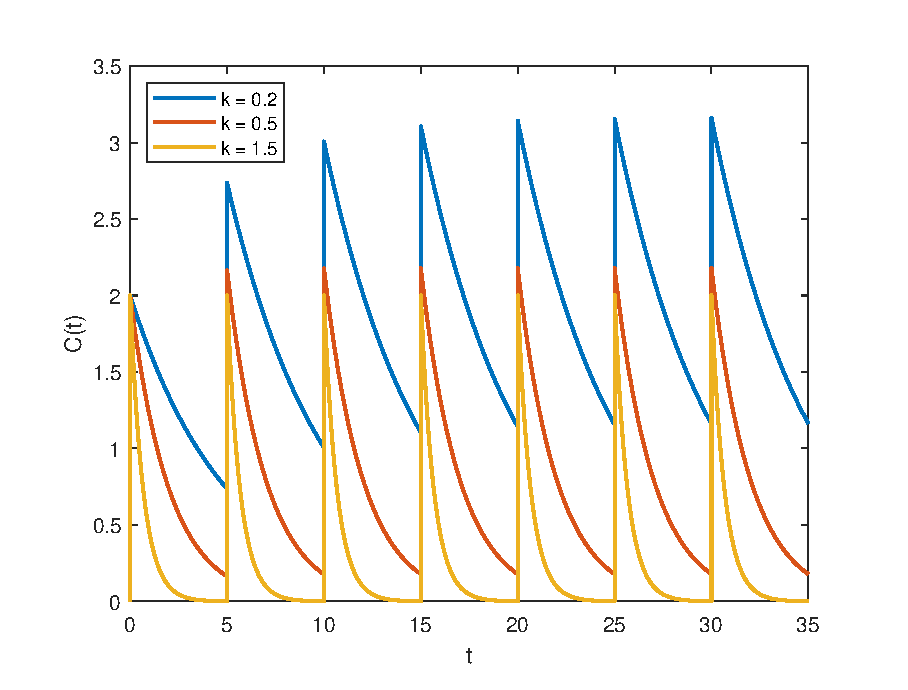
\includegraphics[width=0.5\linewidth]{浓度随时间变化.eps}
    \caption{不同$k$取值下药物浓度随时间变化}
    \label{fig:药物浓度随时间变化}
\end{figure}

从图中我们可以发现:

\begin{itemize*}
    \item $k$的取值决定了药物浓度的降低速率,$k$越大,药物浓度降低的速率越快;
    \item 当$k$的取值较小的时候,药物浓度变化较为平缓,重复服药时,药物浓度尚未降低至0,这导致了药物浓度的累计,随着时间的推移,药物的最低浓度会稳定在一个大于0的值;
    \item 当$k$的取值较大的时候,药物浓度变化较为陡峭,重复服药时,药物浓度已经降低至接近0。每次服药时,药物浓度的变化时相同的。
\end{itemize*}

\subsection{单服药周期内最低与最高药物浓度}

我们对于这个问题,更加关注病人在服药一段时间后,体内药物浓度的最低值与最高值,如果最低值过低,可能会导致药物浓度不足,无法达到治疗效果;如果最高值过高,可能会导致药物浓度过高,对患者造成严重的负面影响。

也就是说,我们其实是关注药物浓度的波动范围,也就是图\ref{fig:上下限}中表示的最低点和最高点两条曲线。

\begin{figure}[!ht]
    \centering
    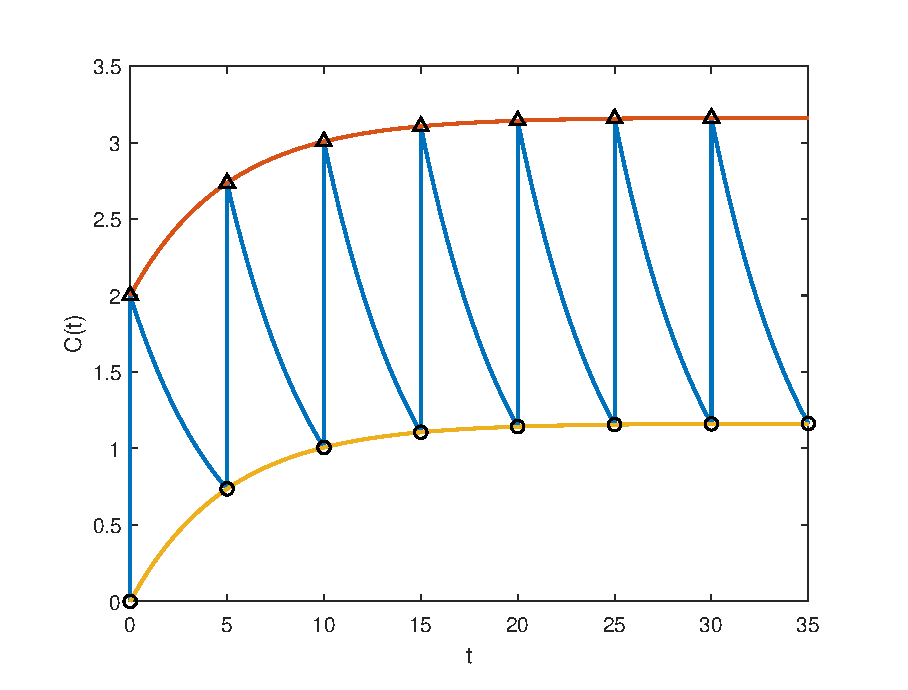
\includegraphics[width=0.5\linewidth]{上下限.eps}
    \caption{药物浓度波动范围示意图}
    \label{fig:上下限}
\end{figure}

不难发现,最高点的曲线就是最低点的曲线加上$A$的偏置,因此,我们在这里只关注最低点的曲线。

我们发现,最低点的取值是一个数列,其中$a_0 = 0$,$a_{n+1} = (a_n + A)\,\mathrm{e}^{-k\,T}$。如果这个数列是收敛的,那么对于极限$a = \lim_{n\to\infty} a_n$,有:

\begin{equation}
    a = (a + A)\,\mathrm{e}^{-k\,T}
\end{equation}

解这个方程,我们可以得到:

\begin{equation}
    a = \frac{A\,\mathrm{e}^{-k\,T}}{1 - \mathrm{e}^{-k\,T}}
\end{equation}

我们接下来论证,这个数列是收敛的:

\begin{enumerate*}
    \item 数列的单调性:我们知道
    \begin{equation}
        a_{n+1}-a_n = A\,\mathrm{e}^{-k\,T} - a_n\,(1 - \mathrm{e}^{-k\,T})
    \end{equation}
    当$a_n < \frac{A\,\mathrm{e}^{-k\,T}}{1 - \mathrm{e}^{-k\,T}}$时,有
    \begin{equation}
        a_n\,(1 - \mathrm{e}^{-k\,T}) < A\,\mathrm{e}^{-k\,T}
    \end{equation}
    因此,当$a_n < \frac{A\,\mathrm{e}^{-k\,T}}{1 - \mathrm{e}^{-k\,T}}$时,有
    \begin{equation}
        a_{n+1}-a_n > 0
    \end{equation}
    也就是
    \begin{equation}
        a_{n+1} > a_n
    \end{equation}
    \item 数列的有界性:我们知道
    \begin{align}
        a_{n+1} - \frac{A\,\mathrm{e}^{-k\,T}}{1 - \mathrm{e}^{-k\,T}} &= (a_n + A)\,\mathrm{e}^{-k\,T} - \frac{A\,\mathrm{e}^{-k\,T}}{1 - \mathrm{e}^{-k\,T}}\\
        &= a_n\,\mathrm{e}^{-k\,T} - \frac{A\,\mathrm{e}^{-2\,k\,T}}{1-\mathrm{e}^{-k\,T}}\\
        &= \mathrm{e}^{-k\,T}\left( a_n - \frac{A\,\mathrm{e}^{-k\,T}}{1 - \mathrm{e}^{-k\,T}}\right)
    \end{align}
    因为,$a_n < \frac{A\,\mathrm{e}^{-k\,T}}{1 - \mathrm{e}^{-k\,T}}$,所以
    \begin{equation}
        a_{n+1} - \frac{A\,\mathrm{e}^{-k\,T}}{1 - \mathrm{e}^{-k\,T}} < 0
    \end{equation}
    也就是
    \begin{equation}
        a_{n+1} < \frac{A\,\mathrm{e}^{-k\,T}}{1 - \mathrm{e}^{-k\,T}}
    \end{equation}
    \item 我们的数列由$a_0 = 0$开始,结合上述讨论,其单调递增,且有上界,由单调有界数列定理,我们知道这个数列是收敛的。且根据上面的讨论:
\end{enumerate*}

综上所述,这个数列是收敛的,且其极限为:
\begin{equation}
    \lim_{n\to\infty} a_n = \frac{A\,\mathrm{e}^{-k\,T}}{1 - \mathrm{e}^{-k\,T}}
\end{equation}

同理不难证明,最高点的取值也是一个数列,记为$b_n$,其中$b_0 = A$,$b_{n+1} = b_n\,\mathrm{e}^{-k\,T} + A$,其极限为:
\begin{equation}
    \lim_{n\to\infty} b_n = \frac{A\,\mathrm{e}^{-k\,T}}{1 - \mathrm{e}^{-k\,T}} + A = \frac{A}{1 - \mathrm{e}^{-k\,T}}
\end{equation}

\subsection{合理的服药剂量与间隔}

经过上面的讨论,我们知道,经过长时间后,每个服药周期内,药物浓度的波动趋于稳定,且其波动范围为$\frac{A\,\mathrm{e}^{-k\,T}}{1 - \mathrm{e}^{-k\,T}}$到$\frac{A}{1 - \mathrm{e}^{-k\,T}}$。

对于病人来说,我们需要保证药物能充分发挥作用,同时又不因为药物浓度过高而导致副作用。因此,我们需要保证药物浓度的最低值不低于一定的阈值$C_{min}$,同时又不高于一定的阈值$C_{max}$。

因此,我们可以得到如下的不等式:
\begin{equation}
    \left\{
        \begin{aligned}
            \frac{A\,\mathrm{e}^{-k\,T}}{1 - \mathrm{e}^{-k\,T}} &\geq C_{min}\\
            \frac{A}{1 - \mathrm{e}^{-k\,T}} &\leq C_{max}
        \end{aligned}
    \right.
\end{equation}

我们先将$\frac{A}{1-\mathrm{e}^{-k\,T}}$看做一个整体,则我们可以得到:
\begin{equation}
    \mathrm{e}^{-k\,T} \geq \frac{C_{min}}{C_{max}}
\end{equation}
观察该式,我们可以发现$\mathrm{e}^{-k\,T}$的物理意义,其是衰减系数,经过时间$T$后,药物浓度会衰减至原本的$\mathrm{e}^{-k\,T}$。我们也可以将这个不等式转化为关于时间$T$的(当然,还有$T > 0$):
\begin{equation}
    T \leq -\frac{\ln\frac{C_{min}}{C_{max}}}{k}
\end{equation}

当我们确定了一个合理的$T$之后,我们可以得到一个合理的$A$的取值范围:
\begin{equation}
    \left\{
        \begin{aligned}
            A &\geq C_{min}\,\frac{1 - \mathrm{e}^{-k\,T}}{\mathrm{e}^{-k\,T}}\\
            A &\leq C_{max}\,(1 - \mathrm{e}^{-k\,T})
        \end{aligned}
    \right.
\end{equation}

我们取$C_{max} = 4$,$C_{min} = 1$,$k = 0.2$,$T = 5$,我们可以绘制出如下示意图\ref{fig:有效取值范围}。其中,封闭曲线所覆盖的区域中的每一个点,都是一个可以保证,经过足够长时间后,浓度在$C_{max}$和$C_{min}$范围内波动的取值。

\begin{figure}[!ht]
    \centering
    \subfloat[单次服药量$A$与衰减系数$\mathrm{e}^{-k\,T}$]{
		\includesvg[width=0.45\linewidth]{合理取值_衰减系数.svg}}
	\subfloat[单次服药量$A$与时间间隔$T$]{
		\includesvg[width=0.45\linewidth]{合理取值_时间.svg}}
    \caption{变量的有效取值范围}
    \label{fig:有效取值范围}
\end{figure}

当然,我们也需要根据实际需要来选取单次服药量和服药时间间隔。虽然图中每一个点都可以保证药物浓度维持在特定范围内,但是显然,过短的服药间隔是不合理的。

\section{总结}

我们在本文中,首先给出了,在给定$k$,$T$,$A$的情况下,病人体内药物浓度随时间变化的情况。之后,通过对数列求极限,得到了足够长时间后,病人体内药物浓度变化范围关于$k$,$T$和$A$的解析表达式。最后,我们在任意给定药物所需的$C_{min}$,$C_{max}$的情况下($k$不变,我们认为其只与药物本身的性质有关),给出了$T$和$A$的合理的取值范围。

\appendix

\section{附录:所用代码}

\subsection*{main.m}

\begin{minted}{matlab}
clearvars
[t1,c1] = showChange(5,2,0.2,7);
[t2,c2] = showChange(5,2,0.5,7);
[t3,c3] = showChange(5,2,1.5,7);

% 绘制不同k取值的图
f1 = figure(1);
plot([0;t1],[0;c1],LineWidth=1.5)
hold on
plot([0;t2],[0;c2],LineWidth=1.5)
plot([0;t3],[0;c3],LineWidth=1.5)
xlabel("t")
ylabel("C(t)")
legend(["k = 0.2","k = 0.5","k = 1.5"],Location="northwest")

% 绘制上限与下限
f2 = figure(2);
t1 = [0;t1]; tmin = t1(1:100:701); tmax = t1(2:100:701);
c1 = [0;c1]; cmin = c1(1:100:701); cmax = c1(2:100:701);
fitModel = fittype(@(a,b,c,x)a.*exp(1 - b.*x)+c, ...
    'independent',{'x'},'coefficients',{'a','b','c'});
fmax = fit(tmax,cmax,fitModel,'StartPoint',[-0.4,0.2,3]);
fmin = fit(tmin,cmin,fitModel,'StartPoint',[-0.4,0.2,3]);
plot(t1,c1,LineWidth=1.5)
hold on
plot(t1,fmax(t1),LineWidth=1.5)
plot(t1,fmin(t1),LineWidth=1.5)
plot(tmin,cmin,'ko',LineWidth=1)
plot(tmax,cmax,'k^',LineWidth=1)
xlabel("t")
ylabel("C(t)")
axis([0 35 0 3.5])

% 计算合理区域
Cmax = 4; Cmin = 1; K = 0.2;
X = zeros(1,200);
X(1:100)   = linspace(Cmin/Cmax,1,100);
X(101:200) = linspace(1,Cmin/Cmax,100);
Y = zeros(1,200);
Y(1:100)   = Cmin .* (1 - X(1:100)) ./ X(1:100);
Y(101:200) = Cmax .* (1 - X(101:200));
T = - log(X) ./ K;

warnState = warning('off', 'all');
% 绘制合理区域
f3 = figure(3);
pgon = polyshape(X,Y,'Simplify',true);
plot(pgon,FaceColor='red',FaceAlpha=0.1,LineWidth=1.5,EdgeColor='red')
xlabel("e^{-kT}")
ylabel("A")
axis([0.25 1 0 3])
box on
%绘制合理区域2
f4 = figure(4);
pgon = polyshape(T,Y,'Simplify',true);
plot(pgon,FaceColor='red',FaceAlpha=0.1,LineWidth=1.5,EdgeColor='red')
xlabel("T")
ylabel("A")
axis([0 7 0 3])
box on
warning(warnState);

% 辅助函数
function [t,Ct] = showChange(T, A, k1, n)
    syms t0 C0 C(x) x k
    s = dsolve(diff(C,x) == -k*C(x), C(t0) == C0);

    npoints = 100;
    Ct = zeros(npoints * n, 1);
    t  = zeros(npoints * n, 1);

    c = 0;
    for i=1:n
        t(npoints*(i-1)+1:npoints*i) = linspace((i-1)*T,i*T).';
        c = c + A;

        s_sub = subs(s,[t0, C0, k], [(i-1)*T, c, k1]);
        s_func = matlabFunction(s_sub);
        Ct(npoints*(i-1)+1:npoints*i) = s_func(t(npoints*(i-1)+1:npoints*i));
        c = Ct(npoints*i);
    end
end
\end{minted}


\end{document}

